\documentclass[journal]{IEEEtran}
\IEEEoverridecommandlockouts

\usepackage{cite}
\usepackage{amsmath,amssymb,amsfonts}
\usepackage{algorithm}
\usepackage{algorithmic}
\usepackage{graphicx}
\graphicspath{{figures/}{./}}
\usepackage{textcomp}
\usepackage{xcolor}
\usepackage{booktabs}
\usepackage{tabularx}
\usepackage{multirow}
\usepackage{array}
\usepackage{makecell}
\usepackage{url}
\usepackage[hidelinks]{hyperref}
\hypersetup{
  pdftitle={SENTINEL: Evasion-Aware Trust Scoring, Deception, and Cryptographic Write Authorization for Industrial IoT - Extended Manuscript},
  pdfauthor={Mohammad Salman Khan, Hammad Chughtai, Halil Ibrahim Ozkul, Burak Yilmaz},
  pdfkeywords={Industrial IoT, operational technology, trust scoring, cyber deception, command authorization}
}
\usepackage{tikz}
\usetikzlibrary{shapes,arrows.meta,positioning}
\definecolor{orcidlogocol}{HTML}{A6CE39}
\newcommand{\orcidicon}[1]{\href{https://orcid.org/#1}{\mbox{
\begin{tikzpicture}[baseline=-0.35em,scale=0.08]
\fill[orcidlogocol] (0,0) circle (1.0);
\draw[white, fill=white] (-0.35,0.55) circle (0.12);
\draw[white, line width=0.25mm] (-0.35,0.3) -- (-0.35,-0.6);
\draw[white, line width=0.25mm] (0.0,0.55) -- (0.0,-0.6);
\draw[white, line width=0.25mm] (0.0,0.55) .. controls (0.5,0.55) and (0.5,0.0) .. (0.0,0.0);
\end{tikzpicture}}}}

\IfFileExists{orcidlink.sty}{
  \usepackage{orcidlink}
  \let\orcid\orcidlink
}{
  \let\orcid\orcidicon
}
\usepackage{microtype}
\usepackage{enumitem}
\setlist{nosep,leftmargin=*}
\renewcommand{\arraystretch}{1.08}

\newcommand{\cmark}{\textcolor{green!50!black}{\checkmark}}
\newcommand{\xmark}{\textcolor{red!65!black}{\texttimes}}
\newcommand{\partialmark}{\textcolor{orange!80!black}{$\triangle$}}
\newcommand{\sentinel}{\textsc{Sentinel}}
\newcommand{\modelb}{Model~B}
\newcommand{\modela}{Model~A}

\DeclareMathOperator{\Sanitize}{Sanitize}
\DeclareMathOperator{\Concat}{Concat}
\DeclareMathOperator{\KDF}{KDF}
\DeclareMathOperator{\Ser}{Ser}
\DeclareMathOperator{\HMAC}{HMAC}
\DeclareMathOperator{\VerifyCap}{VerifyCap}
\DeclareMathOperator{\CheckFreshness}{CheckFreshness}
\DeclareMathOperator{\InitDecoySession}{InitDecoySession}
\DeclareMathOperator{\ForwardWriteToPLC}{ForwardWriteToPLC}
\DeclareMathOperator{\AtomicAdd}{AtomicAdd}
\DeclareMathOperator{\CTCompare}{CT\text{-}Compare}

\begin{document}

\title{SENTINEL: Evasion-Aware Trust Scoring, Deception, and Cryptographic Write Authorization for Industrial IoT}

\author{
\IEEEauthorblockN{Mohammad Salman Khan\,\orcid{0009-0003-5559-669X}\IEEEauthorrefmark{1},
Hammad Chughtai\,\orcid{0009-0006-8040-601X}\IEEEauthorrefmark{2},
Halil \.{I}brahim \"Ozkul\,\orcid{0009-0005-1300-8778}\IEEEauthorrefmark{1}, and
Burak Y\i lmaz\,\orcid{0000-0001-5549-8385}\IEEEauthorrefmark{1}}
\IEEEauthorblockA{\IEEEauthorrefmark{1}Department of Software Engineering, Konya Technical University, Konya, Turkey}
\IEEEauthorblockA{\IEEEauthorrefmark{2}Department of Computer Science (Cyber Security), University of Bradford, Bradford, United Kingdom}
}

\maketitle

\begin{abstract}
Industrial Internet of Things (IIoT) environments require security controls that can distinguish legitimate operational changes from credential misuse, gradual process manipulation, and unauthorized command execution without violating real-time and availability constraints. Detection alone is insufficient when a compromised network-facing service can still issue writes to operational technology. This paper presents SENTINEL, an architecture that separates a public command broker from a protected trust decision point, routes uncertain sessions to a session-isolated deception environment, and requires a short-lived, HMAC-authenticated write capability for every live actuator update. A windowed trust scorer evaluates 152 statistical features across identity, temporal cadence, role authorization, and cross-sensor process consistency. Across five independent runs, each using a newly generated synthetic corpus of 192,000 commands organized into 4,000 sessions, SENTINEL achieved $98.40\% \pm 0.45\%$ accuracy, $97.00\% \pm 0.92\%$ macro-F1, and $99.76\% \pm 0.33\%$ simulated decision-path containment. In an end-to-end Modbus/TCP software testbed, 5,000 attack trials spanning role violation, replay, payload modification, slow drift, and broker retargeting caused no unauthorized modification of the protected OpenPLC register. Valid protected writes achieved a median end-to-end latency of 17.52~ms (P95: 18.56~ms, P99: 18.73~ms), adding 4.06~ms paired median overhead over the unprotected Modbus baseline. These results demonstrate the architectural feasibility of combining continuous behavioral scoring, active deception, and short-lived write authorization to limit unauthorized process manipulation following compromise of a network-facing component.
\end{abstract}

\begin{IEEEkeywords}
Industrial IoT, operational technology, trust scoring, cyber deception, honeypot, command authorization, replay prevention, insider threat, evasion attack.
\end{IEEEkeywords}

\section{Introduction}
Operational technology (OT) increasingly depends on interconnected sensors, programmable logic controllers (PLCs), remote engineering workstations, gateways, and cloud or enterprise services. This convergence improves observability and automation but exposes physical processes to software and identity compromise. OT defenses must therefore protect not only information assets, but also actions that can change a physical process. NIST emphasizes that OT security controls must preserve safety, reliability, and performance requirements that differ from conventional enterprise systems \cite{nist82}.

A recurring weakness in industrial architectures is that a successfully authenticated session is treated as trustworthy for the remainder of its interaction. Stolen credentials, a malicious insider, or a compromised network-facing service can then issue commands that are individually valid but collectively unsafe. Slow manipulation is especially difficult because an adversary can remain within static ranges and spread a process change across many commands. Prior work has shown that stealthy industrial attacks can trade impact against detectability and can evade monitors that consider only isolated observations \cite{urbina2016}.

Three families of defenses address parts of this problem. Network intrusion detection systems, such as Kitsune, model packet-level or channel-level behavior \cite{kitsune}. Multivariate time-series methods capture temporal and cross-sensor relationships \cite{gdn,usad,tranad}. Industrial honeypots, including Conpot, provide deception and intelligence collection \cite{conpot,ics_honeypot_survey}. These approaches are valuable, but they usually operate in a detect-and-alert mode. They do not necessarily ensure that every physical write is authorized by an isolated policy decision point, and they generally do not use deception as an intermediate response to uncertainty.

This paper presents \sentinel, a command-path architecture that combines four controls. First, a public broker cannot independently authorize a write. Second, a protected trust decision point evaluates policy and recent behavioral context. Third, uncertain sessions are transparently redirected to a session-isolated decoy state instead of being immediately blocked. Fourth, approved writes require a short-lived capability token that is bound to the exact worker, role, target, operation, value, nonce, and policy version. The design follows the zero-trust principle that access decisions should be made for the protected resource rather than inferred from network location \cite{nist207}.

The contributions are:
\begin{itemize}
    \item A separation of the network-facing broker, trust decision point, deception environment, and OT enforcement point, with explicit trust boundaries and failure assumptions.
    \item A command-window trust scorer that combines identity, authorization, timing, replay, and process-context evidence and maps risk into \emph{approve}, \emph{deceive}, or \emph{block} outcomes.
    \item A target-bound HMAC capability and one-time nonce protocol that prevents payload substitution, stale-token use, replay, and cross-device token reuse at an OT gateway.
    \item A reproducible session-level simulation study with a shifted held-out test domain, comparative baselines, feature ablations, token misuse tests, and CPU latency measurements.
    \item An empirical end-to-end Modbus/TCP software-testbed evaluation connecting Model~A, Model~B, an enforcement gateway, OpenPLC Runtime, and a simulated water-tank process.
\end{itemize}

The paper deliberately separates three claims that are often conflated in IIoT security research. \emph{Detection} concerns whether a command sequence is recognized as suspicious; \emph{containment} concerns whether uncertain or malicious activity is prevented from reaching the physical process; and \emph{authorization integrity} concerns whether a network-facing compromise can substitute, replay, or redirect an otherwise valid write. This separation allows a system to remain useful even when the classifier is uncertain: a session can be contained in deception without claiming perfect attack attribution.

The remainder of the paper is organized as follows. Section~II reviews temporal detection, industrial deception, and resource-centric authorization. Section~III defines the assets, design goals, adversary capabilities, and safety assumptions. Sections~IV and V present the architecture, algorithms, implementation choices, and deployment patterns. Sections~VI and VII describe the evaluation and testbed results. Sections~VIII and IX discuss security implications, threats to validity, and directions for broader physical-process and industrial deployment validation.

\section{Background and Related Work}
\subsection{Industrial detection and datasets}
Public testbeds and datasets have enabled repeatable ICS security research. SWaT provides a six-stage water-treatment testbed and associated attack data \cite{swat_testbed,swat_dataset}; TON\_IoT provides telemetry and network data for IoT and IIoT intrusion detection \cite{toniot}. These resources are important, but their recorded variables do not directly represent all of the command-authorization fields required by \sentinel, such as worker role, nonce freshness, request target binding, and session-specific deception state. The present study therefore uses a transparent synthetic command generator and treats real-plant validation as future work rather than presenting synthetic results as field performance.

Kitsune demonstrates efficient online network anomaly detection through an ensemble of autoencoders \cite{kitsune}. USAD, GDN, and TranAD model multivariate temporal behavior using adversarial autoencoders, learned graphs, and transformers, respectively \cite{usad,gdn,tranad}. These models focus primarily on anomaly detection. In contrast, \sentinel's primary unit of control is an authenticated command request, and the output is an enforcement decision rather than an alarm alone.

\subsection{Deception and honeypots}
Conpot emulates industrial protocols to collect intelligence on attackers targeting ICS services \cite{conpot}. Surveys show that industrial honeypots can support threat intelligence and defensive experimentation, but also face realism and fingerprinting limitations \cite{ics_honeypot_survey}. Recent work demonstrates that observable network characteristics can reveal ICS honeypots, reinforcing the need to describe deception fidelity conservatively rather than claim indistinguishability \cite{time_to_lie}.

Shadow honeypots combine anomaly detection with isolated execution and discard state changes caused by malicious requests \cite{shadow}. \sentinel{} adopts a related principle at the command-session level: uncertain commands are executed only against a decoy process state, while the live OT state remains unchanged. Unlike a general software shadow, the decoy is integrated with command authorization and an OT write enforcement point.


\subsection{Resource-centric authorization and zero trust}
Zero-trust architecture does not imply that every request must traverse a cloud identity platform; rather, it requires that access to a protected resource be decided from authenticated identity, device, policy, and context instead of network location alone \cite{nist207}. In an IIoT command path, the protected resource is not merely an API endpoint. It is the ability to mutate an actuator, PLC register, configuration parameter, or process setpoint. Consequently, an application-layer ``allow'' decision is insufficient unless a policy enforcement point adjacent to the OT resource verifies the decision.

SENTINEL implements this separation through a narrow write capability. The capability resembles a message authentication code over an immutable command context and is accepted only once during a short validity interval. HMAC provides integrity and source authentication when the decision point and enforcement point can share a protected key \cite{rfc2104}. This mechanism is complementary to anomaly detection: hard authorization rejects commands that are invalid independent of behavior, while the scorer handles context-dependent cases that are individually legal but collectively suspicious.

\subsection{Gap addressed by this work}
The literature contains strong components for network anomaly detection, multivariate process monitoring, deception, and policy enforcement, but these components are usually evaluated independently. A detector may report a suspicious session without controlling whether its next write reaches the plant; a honeypot may attract scanning traffic without being part of a live command decision; and a cryptographic gateway may verify integrity without detecting a legitimate credential being used gradually and maliciously. The research question addressed here is therefore architectural as well as predictive: can these controls be composed into one command lifecycle with measurable trade-offs among availability, uncertainty handling, and write prevention?

\subsection{Positioning}
Table~\ref{tab:positioning} compares the principal capabilities relevant to this work. The table avoids subjective readiness scores; it records whether each work directly supports the listed function.

\begin{table*}[t]
\centering
\caption{Capability positioning of representative approaches}
\label{tab:positioning}
\renewcommand{\arraystretch}{1.15}
\begin{tabularx}{\textwidth}{@{}XcccccX@{}}
\toprule
\textbf{Approach} & \textbf{Command-level context} & \textbf{Temporal behavior} & \textbf{Enforced write gate} & \textbf{Active deception} & \textbf{OT/IIoT focus} & \textbf{Primary role} \\
\midrule
Kitsune \cite{kitsune} & \xmark & \cmark & \xmark & \xmark & \partialmark & Network anomaly detection \\
USAD / GDN / TranAD \cite{usad,gdn,tranad} & \partialmark & \cmark & \xmark & \xmark & \partialmark & Multivariate anomaly detection \\
Conpot \cite{conpot} & \xmark & \xmark & \xmark & \cmark & \cmark & ICS honeypot and intelligence collection \\
Shadow honeypots \cite{shadow} & \partialmark & \partialmark & \xmark & \cmark & \xmark & Isolated validation of suspicious software requests \\
\textbf{SENTINEL} & \cmark & \cmark & \cmark & \cmark & \cmark & Command decision, deception, and write enforcement \\
\bottomrule
\end{tabularx}
\vspace{2pt}
{\footnotesize \cmark~= directly supported; \partialmark~= partial or indirect support; \xmark~= not a native function.}
\end{table*}

\section{System and Threat Model}
\subsection{Design objectives}
The architecture is guided by six objectives. \textbf{G1: mandatory mediation} requires every remote write to pass through a verifier adjacent to the OT resource. \textbf{G2: broker compromise tolerance} requires Model~B to remain unable to create a valid physical-write authorization by itself. \textbf{G3: temporal context} requires the decision point to evaluate a sequence rather than a single command. \textbf{G4: uncertainty containment} requires suspicious but inconclusive sessions to be isolated without immediately disrupting all legitimate activity. \textbf{G5: bounded overhead} requires the decision path to remain compatible with supervisory command rates. \textbf{G6: auditable evidence} requires decisions, token outcomes, and decoy interactions to be reconstructable without automatically poisoning the trusted baseline.

\subsection{Formal system and state-transition model}
We model the OT process as a discrete-time state-transition system over a continuous-valued plant state space:
\begin{equation}
\mathcal{M} = (\mathcal{S}, \mathcal{C}, \delta, s_0),
\end{equation}
where $\mathcal{S} \subseteq \mathbb{R}^d$ denotes the continuous physical plant state space (pressures, flow rates, temperatures, and valve states), $\mathcal{C}$ is the domain of canonical normalized commands, $\delta: \mathcal{S} \times \mathcal{C} \to \mathcal{S}$ is the underlying process dynamics transition function, and $s_0 \in \mathcal{S}$ is the initial plant state.

Let $\mathcal{C}_{\mathrm{write}} \subset \mathcal{C}$ represent the subset of state-mutating commands (setpoint updates or actuator toggles). In traditional, unprotected IIoT deployments, any issued command $c_t \in \mathcal{C}_{\mathrm{write}}$ directly triggers physical state evolution:
\begin{equation}
s_{t+1} = \delta(s_t, c_t).
\end{equation}

\sentinel{} decouples public command ingress from physical state mutation by introducing a dual-namespace state transformation $(\psi_{\mathrm{live}}, \psi_{\mathrm{decoy}}^{(k)})$:
\begin{align}
s_{t+1}^{\mathrm{live}} &= \psi_{\mathrm{live}}\bigl(s_t^{\mathrm{live}}, c_t, T_t\bigr), \\
s_{t+1}^{\mathrm{decoy},(k)} &= \psi_{\mathrm{decoy}}^{(k)}\bigl(s_t^{\mathrm{decoy},(k)}, c_t\bigr),
\end{align}
where $T_t$ is an HMAC-authenticated write capability, and $k \in \mathbb{N}$ denotes a session-isolated decoy namespace. The live state evolution $\psi_{\mathrm{live}}$ enforces the strict verification predicate:
\begin{align}
&\psi_{\mathrm{live}}\bigl(s_t^{\mathrm{live}}, c_t, T_t\bigr) \nonumber \\
&\quad = \begin{cases}
\delta(s_t^{\mathrm{live}}, c_t), & \text{if } \VerifyCap(c_t, T_t, K_{\mathrm{epoch}}) = \mathsf{True}, \\[3pt]
s_t^{\mathrm{live}}, & \text{otherwise}.
\end{cases}
\end{align}

\noindent\textbf{Intuitive Interpretation:} Physical plant actuators and setpoint registers update if and only if a fresh cryptographic capability token $T_t$ is verified at the OT gateway. If an unverified or suspicious command arrives, the live physical process state remains locked ($s_t^{\mathrm{live}}$), while the command is safely redirected to the session-isolated deception layer without causing physical plant disruption.

\subsection{Protected assets and security invariants}
The protected assets are the live actuator/setpoint state, worker authorization context, session decision state, forensic evidence, identity-signing material, and capability-authentication key material. The central invariant is that live OT state changes only after the enforcement point verifies a fresh capability whose authenticated fields exactly match the pending command. Identity is signed independently of Model~B; uncertainty is isolated in a session-specific decoy namespace; audit evidence is append-only; and the broker never possesses the capability HMAC key.

\subsection{System entities}
The architecture contains five security-relevant entities, as illustrated in Fig.~\ref{fig:architecture}:
\begin{enumerate}
    \item \textbf{Ingress identity service.} Authenticates the worker and device, validates request freshness, and produces a signed identity context.
    \item \textbf{Model B, public command broker.} Parses protocol messages, normalizes commands, and maintains session transport state. It does not make final trust decisions.
    \item \textbf{Model A, trust decision point.} Applies hard policy constraints, computes a behavioral score, chooses an action, and generates HMAC-authenticated write capabilities.
    \item \textbf{Deception service.} Maintains a session-isolated decoy state and returns protocol-consistent acknowledgments without changing the live process.
    \item \textbf{OT enforcement point.} Validates the capability, nonce, target, role, value, and expiration before forwarding a write to a PLC, actuator, or legacy gateway.
\end{enumerate}

\begin{figure*}[t]
\centering
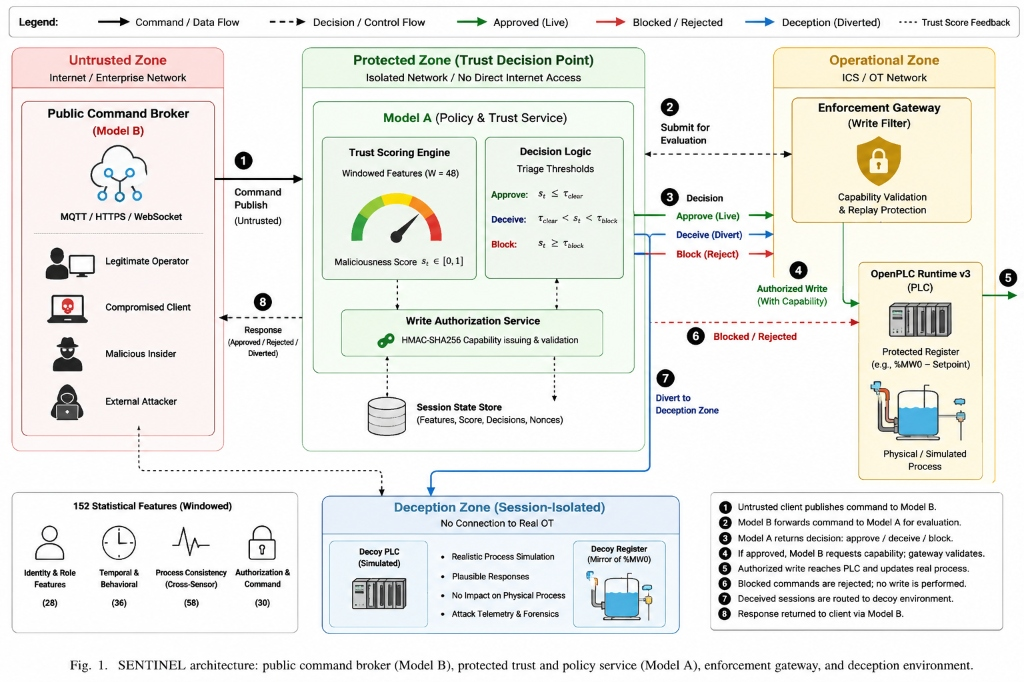
\includegraphics[width=\linewidth]{fig_architecture.png}
\caption{End-to-end SENTINEL command mediation architecture showing the Untrusted Zone with public broker (Model~B), Protected Zone trust decision point (Model~A) with 152 windowed statistical features ($W=48$) and HMAC-SHA256 capability issuance, Operational Zone write enforcement gateway and OpenPLC controller, session-isolated Deception Zone, and numbered 8-step command lifecycle.}
\label{fig:architecture}
\end{figure*}

\subsection{Adversary capabilities and threat model}
We consider five operational attack classes and one architectural compromise. An insider may issue legal commands whose cumulative effect is unsafe; stolen credentials may be used from an unusual origin or cadence; a slow-evasion adversary may spread low-amplitude changes over time; an authenticated worker may exceed role permissions; and a replay attacker may repeat, retarget, or modify captured commands. We also allow arbitrary code execution in Model~B, including payload alteration and reordering.

Assuming the HMAC key remains secret and canonical serialization is unambiguous, an adversary cannot generate a valid capability for a new command without forging HMAC-SHA256. Uniform 128-bit nonces and atomic single-use consumption provide replay resistance and make accidental nonce collision (approximately $q_{\mathrm{cap}}(q_{\mathrm{cap}}-1)/2^{129}$) negligible. Under the stated key-separation assumptions, Model~B alone therefore cannot authorize a new or modified live write.

\subsection{Trusted computing base and exclusions}
The trusted computing base contains Model~A, the capability HMAC key, the OT enforcement point, and the identity-signing service. Physical tampering, compromise of Model~A, compromise of the enforcement gateway, and denial-of-service against the control channel are outside the experimentally evaluated threat model. The behavioral scorer cannot guarantee detection of a perfectly in-distribution attack that produces no measurable identity, temporal, authorization, or process-context deviation. These assumptions follow the adversarial-ML distinction between attacker knowledge, capability, and lifecycle access \cite{nistaml}.

\subsection{Safety and failure behavior}
A security gateway must not replace local safety interlocks. If Model~A is unavailable, remote writes fail closed, while local PLC safety logic, emergency shutdown, and manually authorized maintenance procedures remain independent. Reads may continue through a degraded path when organizational policy permits. A maintenance bypass, when required, must be explicit, time-bounded, physically or independently approved, and logged; it must not be implemented as a silent fail-open condition.

The reference prototype evaluates command integrity and authorization; it does not claim to certify process safety. A production deployment must define the safe state for each actuator, the maximum tolerated decision delay, clock-skew bounds, gateway restart behavior, and what happens to unused capabilities when a policy or key version changes.

\section{SENTINEL Design}
\subsection{End-to-end command lifecycle}
A command passes through eight operational steps grouped into six logical stages, matching the numbered lifecycle in Fig.~\ref{fig:architecture}. First, an ingress identity service authenticates the worker and issues a signed context $I_t$. Second, Model~B parses protocol inputs and publishes canonical command $c_t$ to Model~A. Third, Model~A evaluates hard constraints and windowed trust scores ($s_t$). Fourth, if approved ($s_t < \tau_{\mathrm{clear}}$), Model~A issues capability $T_t$. Fifth, the OT enforcement gateway verifies $T_t$ and updates the OpenPLC register. Sixth, commands failing hard checks or exceeding $\tau_{\mathrm{block}}$ are blocked. Seventh, suspicious sessions ($\tau_{\mathrm{clear}} \le s_t < \tau_{\mathrm{block}}$) are diverted to deception. Eighth, execution status is returned to the client via Model~B. No response from Model~B alone is sufficient to mutate the live physical state.

\subsection{Command context and hard constraints}
A normalized command at time $t$ is represented as
\begin{equation}
 c_t = (u, r, d, o, v, n, t_i, t_e, p),
\end{equation}
where $u$ is the worker identity, $r$ the role, $d$ the target device or register, $o$ the operation, $v$ the value, $n$ a nonce, $t_i$ and $t_e$ the issue and expiry times, and $p$ the policy version. Before behavioral scoring, Model~A rejects malformed requests, stale identity contexts, role violations, unsafe values, and operations outside the target policy. Hard violations are never routed to the live process.

The policy evaluation order is intentional. Syntax and freshness checks occur before any expensive model operation. Role and target authorization then establish whether the operation is categorically permitted. A device-specific safe envelope rejects values that are unacceptable regardless of behavioral history. Only a command that is individually admissible proceeds to contextual scoring. This arrangement avoids using a probabilistic model to override deterministic safety or authorization rules.

During session startup, before 48 commands are available, Model~A pads the window by repeating the initial command state. As new observations arrive, padded entries are progressively evicted. Deterministic authorization and safety constraints remain active throughout startup and are never relaxed.

\subsection{Command-window feature construction}
For commands that satisfy hard constraints, Model~A maintains a sliding session window of the $W=48$ most recent observations for each worker session $S_t = (c_{t-W+1}, \dots, c_t)$. During startup, before $W$ commands accumulate, the window is padded by repeating the initial state; as new commands arrive, padded entries are evicted. From this matrix, Model~A constructs a 152-dimensional summary vector $\phi(S_t)$ spanning eight temporal statistics across 19 base command features.

For each feature channel $j \in \{1,\dots,19\}$, the extraction operator $\Phi_j(S_t) \in \mathbb{R}^8$ evaluates eight temporal summary statistics (mean $\mu_j$, standard deviation $\sigma_j$, minimum, maximum, end-to-start difference $\Delta_j = c_{t,j} - c_{t-W+1,j}$, linear slope $\nabla_j$, first quartile $Q1_j$, and third quartile $Q3_j$). The linear slope $\nabla_j$ is calculated via ordinary least-squares regression:
\begin{equation}
\nabla_j = \frac{\sum_{k=1}^W (k - \bar{k})(c_{t-W+k,j} - \mu_j)}{\sum_{k=1}^W (k - \bar{k})^2}, \quad \bar{k} = \frac{W+1}{2}.
\end{equation}
Concatenating these operators across all 19 feature channels yields the complete session summary vector:
\begin{align}
\Phi_j(S_t) &= \begin{bmatrix} \mu_j & \sigma_j & \min_j & \max_j & \Delta_j & \nabla_j & Q1_j & Q3_j \end{bmatrix}^T, \\
\phi(S_t) &= \Concat\bigl( \Phi_1(S_t), \Phi_2(S_t), \dots, \Phi_{19}(S_t) \bigr) \in \mathbb{R}^{152}.
\end{align}

Table~\ref{tab:features} groups the command-level evidence by security purpose.

\begin{table*}[t]
\centering
\caption{Command-level features aggregated over the 48-command session window}
\label{tab:features}
\renewcommand{\arraystretch}{1.12}
\begin{tabularx}{\textwidth}{@{}l l X@{}}
\toprule
\textbf{Group} & \textbf{Features} & \textbf{Security interpretation} \\
\midrule
Operation and target & read/write/setpoint indicators; pump/valve/heater indicators & Distinguishes ordinary monitoring from state-changing operations and captures device-specific patterns \\
Process context & normalized value, normalized delta, cross-sensor residual, safe-envelope flag & Detects cumulative drift and inconsistency between a requested value and related process observations \\
Identity and authorization & role-permission flag, origin-trust score & Identifies commands that conflict with the role or appear from an unusual authenticated context \\
Freshness and replay & nonce-freshness flag, repeated-command similarity & Captures stale or duplicated command material and replay-like sequences \\
Timing and workload & log inter-arrival time, rate deviation, time-of-day sine/cosine & Models cadence, bursts, shift changes, and unusual access times without treating one time value as categorically malicious \\
Session position & normalized session progress & Allows the scorer to distinguish benign startup/maintenance transients from evidence that emerges late in a session \\
\bottomrule
\end{tabularx}
\end{table*}

Within the process-context feature group, cross-sensor consistency is continuously tracked via an Exponentially Weighted Moving Average (EWMA) residual $\hat{r}_t$, while operational diversity is measured using Shannon entropy $H(O_t)$:
\begin{align}
\hat{r}_t &= \beta \hat{r}_{t-1} + (1-\beta) |v_t - f_{\mathrm{phys}}(x_t)|, \\
H(O_t) &= -\sum_{o \in \mathcal{O}} p(o) \log_2 p(o),
\end{align}
where $f_{\mathrm{phys}}(x_t)$ estimates expected setpoint response from correlated sensor readings $x_t$, $\beta \in (0,1)$ is a smoothing factor, and $p(o)$ is the empirical probability of operation $o$ within window $S_t$.

\noindent\textbf{Physical Feature Interpretation:} Each aggregated feature component captures a distinct physical attack footprint:
\begin{itemize}
    \item \textbf{Linear Slope ($\nabla_j$):} Detects rapid or stealthy incremental setpoint manipulation over time.
    \item \textbf{EWMA Residual ($\hat{r}_t$):} Quantifies physical inconsistency between requested setpoints $v_t$ and expected plant telemetry $f_{\mathrm{phys}}(x_t)$.
    \item \textbf{Shannon Entropy ($H(O_t)$):} Measures operational diversity, spotting automated polling loops or unnatural command repetition.
\end{itemize}

Evasion awareness arises from training and evaluating the scorer on gradual, low-amplitude manipulation sequences, together with temporal slope, cumulative-delta, cadence, and cross-sensor residual features; it does not imply certified adversarial robustness. Startup-window behavior is treated as a limitation because repeating the initial command state during startup produces feature distributions that differ from mature windows.

The deployed reference scorer is a 160-tree random forest with maximum depth 15, minimum leaf size 3, square-root feature sampling, and balanced subsampling. A tree ensemble was selected over a recurrent model because it provided stronger shifted-test performance and interpretable feature importance in the reference study.

Let $P(y=k\mid \phi(S_t))$ be the class probability for the current session summary $\phi(S_t)$. The maliciousness score is
\begin{equation}
 s_t = 1 - P(y = \mathrm{normal} \mid \phi(S_t)).
\end{equation}
The response is
\begin{equation}
 D(s_t) =
 \begin{cases}
 \mathrm{approve}, & s_t < \tau_{\mathrm{clear}}, \\[2pt]
 \mathrm{deceive}, & \tau_{\mathrm{clear}} \le s_t < \tau_{\mathrm{block}}, \\[2pt]
 \mathrm{block}, & s_t \ge \tau_{\mathrm{block}}.
 \end{cases}
\end{equation}
Thresholds are selected on the validation set under a constraint that immediate false blocks remain below 2\%. Candidate pairs are ranked using
\begin{equation}
U = 1.6\,C_a + 0.8\,A_b + 0.25\,B_a - 3.2\,B_b,
\end{equation}
where $C_a$ is attack containment, $A_b$ is benign approval, $B_a$ is immediate attack blocking, and $B_b$ is benign immediate blocking. Utility coefficients and candidate threshold ranges were specified on the validation set prior to evaluation on the held-out test set; the test partition was not used for weight tuning or threshold selection. The selected values are $\tau_{\mathrm{clear}} = 0.45$ and $\tau_{\mathrm{block}} = 0.65$.

\subsection{Deception state algebra and session transitions}
The deception service allocates a state namespace per suspicious session. On the first diversion at command index $t_{\mathrm{div}}$, the decoy state is initialized via a snapshot operator:
\begin{equation}
s_0^{\mathrm{decoy}, k} = \Sanitize\bigl(s_{t_{\mathrm{div}}}^{\mathrm{live}}\bigr),
\end{equation}
where $\Sanitize$ decouples the decoy state from live actuator registers, removes administrative credentials and historian metadata, and resets physical sensor accumulators while retaining non-sensitive setpoints and process telemetry. Subsequent reads and writes from session $k$ are resolved against that isolated namespace:
\begin{equation}
s_{t+1}^{\mathrm{decoy}, k} = g_{\mathrm{plant}}(s_t^{\mathrm{decoy}, k}, c_t),
\end{equation}
where $g_{\mathrm{plant}}$ simulates protocol-consistent state updates without updating $s^{\mathrm{live}}$. The differential process divergence between live and decoy states is tracked as:
\begin{equation}
\Delta_{\mathrm{decoy}}(t) = \left\| s_t^{\mathrm{live}} - s_t^{\mathrm{decoy}, k} \right\|_2.
\end{equation}

\subsection{Deception mechanics and timing equalization}
When a session produces score $s_t \in [\tau_{\mathrm{clear}}, \tau_{\mathrm{block}})$, Model~A routes the connection to a session-isolated deception worker. The worker maintains decoy state $\psi_{\mathrm{decoy}}^{(k)}$ initialized from benign operational values and returns protocol-compliant responses.

To reduce simple timing distinguishability between the live and decoy paths, the deception gateway samples an additional delay from a non-negative empirical latency distribution collected from the live OT gateway:
\begin{equation}
t_{\mathrm{resp}} = t_{\mathrm{proc}} + \max\left(0, \widetilde{L}_{\mathrm{live}} - t_{\mathrm{proc}}\right),
\end{equation}
where $\widetilde{L}_{\mathrm{live}}$ is sampled from measured live-path latency traces and $t_{\mathrm{proc}}$ is the decoy processing time. This mechanism does not guarantee resistance to advanced timing analysis, but is intended to reduce obvious timing discrepancies while maintaining session-consistent responses.

\noindent\textbf{Operational Mechanics:} Suspicious sessions receive realistic protocol status responses and consistent read-after-write values from $g_{\mathrm{plant}}$, combined with calibrated round-trip timing jitter. This is intended to preserve protocol and read-after-write consistency while reducing obvious timing differences between the live and decoy paths. Decoy responses do not alter the live physical-process state.

The session remains in deception until one of four events occurs: the score crosses $\tau_{\mathrm{block}}$, the session expires, an operator explicitly terminates it, or a de-escalation policy confirms sufficient benign evidence. The reference experiment evaluates diversion and block decisions at the session level; it does not claim a complete industrial process simulator. The decoy is therefore not described as indistinguishable from a real plant. Its purpose is controlled observation and containment. Raw decoy interactions are stored as forensic evidence and are not automatically added to trusted training data, avoiding a direct poisoning path.

\subsection{Capability generation and structure}
For an approved command $c_t$, Model~A generates a short-lived write capability:
\begin{subequations}
\begin{align}
 K_{\mathrm{epoch}} &= \KDF(K_{\mathrm{master}}, \mathrm{epoch} \parallel p), \\
 T_t &= \HMAC_{K_{\mathrm{epoch}}}\bigl(\Ser(u, r, d, o, v, n, t_i, t_e, p)\bigr).
\end{align}
\end{subequations}
The reference lifetime is $\Delta t_{\mathrm{expire}} = t_e - t_i = 800$~ms. The enforcement point recomputes the HMAC, verifies the exact target and value, checks role and safe-envelope constraints, validates the policy version and time interval, and rejects any previously used nonce. A token for one device, value, or operation cannot authorize another. HMAC is used in the reference prototype for low overhead; production deployments may use asymmetric capabilities or hardware-protected keys when organizational key distribution requires them.

\begin{algorithm}[t]
\caption{SENTINEL command decision and capability issuance}
\label{alg:decision}
\begin{algorithmic}[1]
\REQUIRE command $c_t$, signed identity context $I_t$, session history $S_t$, master key $K_{\mathrm{master}}$
\IF{$I_t$ is invalid or $\CheckFreshness(I_t) = \mathsf{False}$}
    \STATE \textbf{return} $\mathsf{Block}$ and append audit alert
\ENDIF
\IF{$c_t$ violates role $r$, target $d$, or safe envelope $[v_{\min}, v_{\max}]$}
    \STATE \textbf{return} $\mathsf{Block}$ and log policy violation
\ENDIF
\STATE append $c_t$ and feature vector to session window $S_t$
\STATE extract 152-dimensional summary vector $\phi(S_t)$
\STATE $s_t \leftarrow 1 - P(y = \mathrm{normal} \mid \phi(S_t))$ using the random-forest ensemble
\IF{$s_t < \tau_{\mathrm{clear}}$}
    \STATE $K_{\mathrm{epoch}} \gets \KDF(K_{\mathrm{master}}, \mathrm{epoch} \parallel p)$
    \STATE $T \gets \HMAC_{K_{\mathrm{epoch}}}(u \parallel r \parallel d \parallel o \parallel v \parallel n \parallel t_i \parallel t_e \parallel p)$
    \STATE \textbf{return} $\mathsf{Approve}$ with capability $T$
\ELSIF{$s_t < \tau_{\mathrm{block}}$}
    \STATE $\mathcal{S}_{\mathrm{decoy}}^{(k)} \gets \InitDecoySession(k, c_t)$
    \STATE \textbf{return} $\mathsf{Deceive}$ via session-isolated decoy state
\ELSE
    \STATE \textbf{return} $\mathsf{Block}$, persist evidence record, and alert SOC
\ENDIF
\end{algorithmic}
\end{algorithm}

\begin{algorithm}[t]
\caption{OT enforcement-point verification}
\label{alg:verify}
\begin{algorithmic}[1]
\REQUIRE pending command $c$, capability $T$, system clock $t$, nonce cache $N_{\mathrm{used}}$, epoch key $K_{\mathrm{epoch}}$
\IF{$T = \emptyset$ or key identifier is unknown}
    \STATE \textbf{return} $\mathsf{Reject}(\text{"Missing token"})$
\ENDIF
\IF{$t < t_i - \Delta t_{\mathrm{skew}}$ or $t > t_e$}
    \STATE \textbf{return} $\mathsf{Reject}(\text{"Expired/Stale token"})$
\ENDIF
\IF{$n \in N_{\mathrm{used}}$ or policy version $p$ is inactive}
    \STATE \textbf{return} $\mathsf{Reject}(\text{"Replay or Inactive Policy"})$
\ENDIF
\IF{$r, d, o, v$ violates local static safety bounds}
    \STATE \textbf{return} $\mathsf{Reject}(\text{"Local Safety Violation"})$
\ENDIF
\STATE $T' \gets \HMAC_{K_{\mathrm{epoch}}}(u \parallel r \parallel d \parallel o \parallel v \parallel n \parallel t_i \parallel t_e \parallel p)$
\IF{$\CTCompare(T', T) \neq \mathsf{Equal}$}
    \STATE \textbf{return} $\mathsf{Reject}(\text{"Capability Authentication Mismatch"})$
\ENDIF
\STATE $\AtomicAdd(N_{\mathrm{used}}, n)$
\STATE $\ForwardWriteToPLC(d, o, v)$
\STATE \textbf{return} $\mathsf{Accept}$ and record audit log
\end{algorithmic}
\end{algorithm}

\subsection{Security properties}
Under the stated trust assumptions, the command path provides four bounded properties. \textbf{P1: exact-command integrity.} Modification of any bound field causes the enforcement point's recomputed HMAC to differ. \textbf{P2: single-use freshness.} A captured capability cannot be accepted after expiry or after its nonce has been atomically consumed. \textbf{P3: broker non-authority.} Model~B cannot independently authorize a write because it lacks the capability HMAC key and cannot produce an independently signed ingress identity context. \textbf{P4: uncertain-write isolation.} A deceive decision resolves the command against a session-specific namespace and therefore does not mutate live OT state.

These are implementation-level properties, not a proof of whole-system safety. They depend on key confidentiality, correct canonical serialization, atomic nonce handling, enforcement-point integrity, and the assumption that all remote writes are mediated. The design does not prevent a local physical override or a compromised PLC from altering its own state.

\subsection{Computational and storage complexity}
Let $W$ be the session-window length, $F$ the number of command features, and $M$ the number of trees. Updating the fixed-window statistics is $O(F)$ with incremental aggregates or $O(WF)$ when recomputed as in the reference script. Tree inference is $O(MD)$ for average tree depth $D$. The reference values $W=48$, $F=19$, $M=160$, and $D\leq15$ keep the path small enough for supervisory traffic. Per-session state consists of the recent command window, the current decision mode, decoy values when applicable, and a bounded set of unexpired nonces.

\section{Reference Implementation and Deployment}
\subsection{Software components}
The reproducibility package implements the synthetic generator, feature aggregation, model training, threshold selection, capability tests, and latency benchmark in Python. The implementation stores each complete session as a $48\times19$ tensor and exports the baseline-specific preprocessing objects, class map, and trained random-forest model in one versioned artifact. The token verifier uses canonical field ordering and constant-time MAC comparison. Random seeds, split rules, model hyperparameters, and generated result files are included so that the reported synthetic experiment can be reproduced.

A production implementation can separate these functions by language and host without changing the protocol. Model~B may be an HTTP, MQTT, OPC UA, or Modbus-facing adapter; Model~A may run as an isolated policy service; and the enforcement point may be embedded in a protocol gateway. The critical requirement is not a specific framework but preservation of the trust boundaries and exact command binding.

\subsection{Deployment patterns}
Two deployment patterns are considered. In a \emph{native-verifier} deployment, a capable PLC, secure edge controller, or actuator firmware validates the capability directly. This minimizes the distance between the protected state and the enforcement logic but requires firmware support and secure key storage. In a \emph{legacy-gateway} deployment, a dedicated gateway is the only routable writer to a legacy PLC. The gateway validates the capability and then emits the protocol-specific command. This is easier to integrate but expands the trusted computing base to include the gateway and the network segment between gateway and PLC.

\subsection{Key, nonce, and policy lifecycle}
Capabilities include a key identifier and policy version so that rotation can occur without accepting commands under an ambiguous policy. During key rotation, the enforcement point may temporarily accept the current and immediately previous key identifiers, subject to their original short expirations. Nonces must be consumed atomically before forwarding the live write; otherwise concurrent duplicate submissions could race. A restart-safe implementation persists or reconstructs all still-valid nonces, or invalidates all outstanding capabilities by advancing the key or policy version.

Audit records should contain the canonical command hash, identity-context identifier, model version, score, selected action, capability identifier, verifier result, and monotonic event time. Sensitive worker identifiers can be pseudonymized in analytical exports while remaining recoverable under controlled incident-response procedures.

\section{Experimental Methodology}
\subsection{Research questions}
The evaluation addresses five questions:
\begin{itemize}
    \item RQ1: Can the scorer distinguish normal sessions from five command-level attack classes under a shifted test domain?
    \item RQ2: What is the operational trade-off among approval, deception, and immediate block thresholds?
    \item RQ3: Does the capability verifier reject common token and payload misuse cases?
    \item RQ4: Is the in-process decision path compatible with low-millisecond command handling?
    \item RQ5: Does the complete SENTINEL command path prevent unauthorized Modbus/TCP writes and remain operationally feasible in an end-to-end software testbed?
\end{itemize}

\subsection{Synthetic command corpus}
The corpus contains 4,000 complete sessions and 192,000 commands. Sixty percent of sessions are normal; each of five attack classes contributes 8\%. Attack sessions begin after a benign prefix and then introduce one of the following patterns:
\begin{itemize}
    \item \textbf{Insider drift:} gradual setpoint change with increasing cross-sensor residual.
    \item \textbf{Credential misuse:} origin and cadence mismatch with mostly valid values.
    \item \textbf{Slow evasion:} low-amplitude cumulative drift that remains within a static safe envelope.
    \item \textbf{Privilege abuse:} intermittent writes outside the worker role.
    \item \textbf{Replay:} repeated commands with stale nonces and elevated similarity.
\end{itemize}
Normal sessions include remote-maintenance, process-transient, and repeated-polling episodes so that single anomalous features are not sufficient for classification. Each session has a randomized role, device type, starting value, cadence, start hour, origin-trust baseline, and read/write/setpoint distribution. Attack onset is sampled between commands 20 and 33 in the base generator, ensuring a benign prefix. Table~\ref{tab:attackgen} summarizes the evidence injected by each attack template. Values are clipped to a normalized range and static unsafe-envelope violations are deliberately rare in the drift classes; this prevents a simple range rule from solving the task.

\begin{table*}[t]
\centering
\caption{Synthetic attack templates and discriminating evidence}
\label{tab:attackgen}
\renewcommand{\arraystretch}{1.12}
\begin{tabularx}{\textwidth}{@{}lXXX@{}}
\toprule
\textbf{Class} & \textbf{Generated behavior after onset} & \textbf{Primary evidence available to scorer} & \textbf{Why a static rule is insufficient} \\
\midrule
Insider drift & Incremental setpoint movement and gradually increasing process residual & Value slope, end-to-start change, residual trend and dispersion & Most individual values remain within the safe envelope and originate from a permitted worker \\
Credential misuse & Lower/more variable origin trust, cadence change, modest workload-rate increase & Origin-trust minimum/trend, inter-arrival statistics, rate deviation & Command syntax, role, and values are usually valid \\
Slow evasion & Smaller cumulative drift with oscillation and weak residual growth & Long-window value and residual slopes & Each update is intentionally below a conspicuous per-command threshold \\
Privilege abuse & Intermittent write/setpoint operations for which role permission is false & Role-permission minimum and variation, operation mix & Violations are sparse and can be surrounded by ordinary reads \\
Replay & Repeated operation/value templates, stale nonces, elevated similarity & Nonce freshness and repeated-command statistics & Replayed commands may contain otherwise safe and historically common values \\
\bottomrule
\end{tabularx}
\end{table*}

The split is stratified by complete session: 70\% training, 15\% validation, and 15\% testing. No command window from one session appears in more than one split. The test set is further shifted by delaying attack evidence, mixing attack traces with independent benign profiles, and injecting mild maintenance-like features into some normal sessions. This shift is intentionally modest: it tests whether the classifier survives overlap and later evidence, but it is not equivalent to an independently collected plant. Table~\ref{tab:dataset} summarizes the split.

\begin{table}[t]
\centering
\caption{Synthetic session corpus distribution}
\label{tab:dataset}
\renewcommand{\arraystretch}{1.12}
\begin{tabular}{@{}lrrrr@{}}
\toprule
\textbf{Class} & \textbf{Total} & \textbf{Train} & \textbf{Val.} & \textbf{Test} \\
\midrule
Normal & 2400 & 1680 & 360 & 360 \\
Insider drift & 320 & 224 & 48 & 48 \\
Credential misuse & 320 & 224 & 48 & 48 \\
Slow evasion & 320 & 224 & 48 & 48 \\
Privilege abuse & 320 & 224 & 48 & 48 \\
Replay & 320 & 224 & 48 & 48 \\
\midrule
\textbf{Total sessions} & \textbf{4000} & \textbf{2800} & \textbf{600} & \textbf{600} \\
\bottomrule
\end{tabular}
\end{table}

\subsection{Baselines and hyperparameters}
We compare the SENTINEL scorer against fixed rules, balanced multinomial logistic regression, and histogram gradient boosting. All learned models use the same 152-dimensional session summaries and the same session splits. Table~\ref{tab:hyperparameters} records the configuration used in the reproducibility package. The rules baseline uses hand-written thresholds on role violations, origin trust, nonce freshness, repeated-command similarity, value drift, process residual, and rate deviation. It represents a plausible low-complexity alternative rather than a published system whose input representation differs from the command corpus.

\begin{table}[t]
\centering
\caption{Evaluated model configurations}
\label{tab:hyperparameters}
\renewcommand{\arraystretch}{1.12}
\begin{tabularx}{\columnwidth}{@{}lX@{}}
\toprule
\textbf{Model} & \textbf{Configuration} \\
\midrule
Rules & Seven feature-derived threshold conditions; first matching attack label returned \\
Logistic regression & Multinomial, balanced class weights, $C=1.2$, maximum 700 iterations \\
Histogram boosting & 180 iterations, learning rate 0.07, 25 maximum leaf nodes, $L_2=0.15$, balanced weights \\
SENTINEL random forest & 160 trees, depth 15, minimum leaf 3, square-root feature sampling, balanced subsampling \\
\bottomrule
\end{tabularx}
\end{table}

\subsection{Performance metrics}
Standard classification metrics—accuracy, macro-precision, macro-recall, macro-F1, balanced accuracy, and benign false-positive rate (FPR)—are calculated on the held-out test set. Although the online scorer produces a decision after each command arrival, classification metrics are calculated from the terminal session prediction. We distinguish two levels of containment. \textbf{Simulated decision-path containment} is recorded in the synthetic evaluation when no malicious command is assigned live approval before the session is diverted or blocked. \textbf{Physical containment} is recorded in the executable Modbus/OpenPLC testbed only when register readback confirms that no unauthorized command modified protected live state. Precision and recall are macro-averaged across all six classes to prevent the larger normal class from dominating reported performance. Binary ROC-AUC and PR-AUC treat all five attack classes as a single positive class to evaluate benign vs. malicious separation.

To express test-set sampling uncertainty, we perform 2,000 nonparametric bootstrap resamples of the 600 held-out sessions and report percentile 95\% confidence intervals for accuracy, macro-F1, FPR, and attack containment. These intervals do not capture generator uncertainty, model-development choices, or deployment shift; they quantify only resampling uncertainty within the fixed test corpus.

\subsection{Capability and latency tests}
The verifier is evaluated using a parameterized test suite containing 14,000 generated misuse cases (2,000 attempts for each of seven misuse patterns: missing token, modified value, expired token, wrong target, replayed nonce, unauthorized role, and unsafe value). A valid control case is executed first. Each negative case changes one relevant condition while preserving the others, allowing the rejection reason to be attributed to the corresponding verification step.

Latency is measured on an AMD EPYC 9V74 virtual host with five vCPUs and 5.9~GiB RAM using Python 3.13 and scikit-learn 1.8. The scorer benchmark uses one model thread after warm-up; the shared preprocessing and scoring pipeline uses 1,000 invocations. HMAC issue and verification are measured separately. Measurements exclude network transport, queueing, database access, audit persistence, protocol translation, and PLC response time. The reported values are therefore computational microbenchmarks rather than end-to-end plant latency.

\subsection{Reproducibility protocol}
The artifact records the random seed, generated class counts, complete-session split, trained model, feature names, threshold values, per-class metrics, ablations, token outcomes, latency samples, and figure-generation scripts. The artifact additionally contains the Modbus/TCP testbed implementation, OpenPLC configuration, process-register map, scenario definitions, raw per-trial latency and register-readback records, environment manifest, and scripts that regenerate the testbed tables. Re-running the package regenerates the synthetic corpus and testbed figures rather than relying on manually entered tables.

\section{Results}
\subsection{Classification performance (Within-Generator Shifted Evaluation)}
Table~\ref{tab:mainresults} reports the shifted-test results under within-generator evaluation. Across 600 held-out shifted test sessions, the SENTINEL scorer achieves 98.50\% accuracy, 97.40\% macro-F1, and a 0.28\% FPR. Gradient boosting achieves 97.83\% accuracy and 95.80\% macro-F1, while the linear and rule baselines fail to separate several temporally overlapping classes. The high binary AUC values should be interpreted alongside the lower multiclass macro-F1: distinguishing attack from normal is easier than identifying the exact attack type.

\begin{table*}[t]
\centering
\caption{Shifted-test classification results (\%)}
\label{tab:mainresults}
\renewcommand{\arraystretch}{1.15}
\begin{tabularx}{\textwidth}{@{}Xrrrrrrrr@{}}
\toprule
\textbf{Model} & \textbf{Acc.} & \textbf{Bal. Acc.} & \textbf{Macro-P} & \textbf{Macro-R} & \textbf{Macro-F1} & \textbf{FPR} & \textbf{ROC-AUC} & \textbf{PR-AUC} \\
\midrule
Rules only & 60.17 & 17.01 & 27.21 & 17.01 & 13.60 & 0.00 & -- & -- \\
Logistic regression & 64.67 & 33.01 & 54.59 & 33.01 & 25.79 & 6.11 & 92.66 & 90.15 \\
Gradient boosting & 97.83 & 95.14 & 96.50 & 95.14 & 95.80 & 0.28 & 99.91 & 99.88 \\
\textbf{SENTINEL scorer} & \textbf{98.50} & \textbf{97.18} & \textbf{97.40} & \textbf{97.18} & \textbf{97.40} & \textbf{0.28} & \textbf{99.88} & \textbf{99.85} \\
\bottomrule
\end{tabularx}
\end{table*}


Bootstrap intervals in Table~\ref{tab:ci} show that the headline result remains high under resampling of the representative seed ($20260724$), with macro-F1 showing expected sampling variation due to 48 test sessions per attack class.

\begin{table}[t]
\centering
\caption{Session-bootstrap 95\% confidence intervals (Seed 20260724)}
\label{tab:ci}
\renewcommand{\arraystretch}{1.12}
\begin{tabular}{@{}lrrr@{}}
\toprule
\textbf{Metric} & \textbf{Point} & \textbf{Lower} & \textbf{Upper} \\
\midrule
Accuracy (\%) & 98.50 & 97.50 & 99.33 \\
Macro-F1 (\%) & 97.40 & 95.80 & 98.67 \\
Benign FPR (\%) & 0.28 & 0.00 & 0.83 \\
Simulated containment (\%) & 99.18 & 98.20 & 99.80 \\
\bottomrule
\end{tabular}
\end{table}

Evaluating class-level recall on seed $20260724$, replay sessions achieve 100.0\% recall, credential misuse 97.9\%, privilege abuse 97.9\%, slow evasion 95.8\%, and insider drift 91.7\%. Figure~\ref{fig:confusion_matrix} illustrates the multi-class confusion matrix on the shifted test set.

\begin{figure}[!ht]
\centering

\includegraphics[width=0.92\columnwidth]{fig_confusion_matrix}
\caption{Shifted-test multi-class confusion matrix for the \sentinel{} random forest scorer across the six evaluated session classes.}
\label{fig:confusion_matrix}
\end{figure}

The score distribution shows strong benign/attack separation, as illustrated in Fig.~\ref{fig:score_dist}, with a small overlap near the clear threshold for credential-misuse, slow-evasion, and privilege-abuse sessions. This overlap motivates a deception band rather than an all-or-nothing classifier threshold.

\begin{figure}[!ht]
\centering

\includegraphics[width=0.95\columnwidth]{fig_score_distribution}
\caption{Distribution of maliciousness score $s_t$ for normal and attack sessions showing the clear threshold ($\tau_{\mathrm{clear}} = 0.45$), block threshold ($\tau_{\mathrm{block}} = 0.65$), and the intermediate deception zone.}
\label{fig:score_dist}
\end{figure}

\subsection{Triage behavior}
At $\tau_{\mathrm{clear}} = 0.45$ and $\tau_{\mathrm{block}} = 0.65$, 99.17\% of benign sessions are approved, 0.83\% enter deception, and none are immediately blocked. Among attack sessions, 99.17\% achieve simulated decision-path containment: 95.00\% are immediately blocked, 4.17\% enter deception, and 0.83\% are approved (Table~\ref{tab:triageclass}). This demonstrates that the two-threshold policy exposes an operational trade-off that a single threshold would hide.

\begin{table}[t]
\centering
\caption{Decision distribution by true class (\%) for Seed 20260724}
\label{tab:triageclass}
\renewcommand{\arraystretch}{1.12}
\begin{tabular}{@{}lrrr@{}}
\toprule
\textbf{Class} & \textbf{Approve} & \textbf{Deceive} & \textbf{Block} \\
\midrule
Normal & 99.17 & 0.83 & 0.00 \\
Insider drift & 0.00 & 8.33 & 91.67 \\
Credential misuse & 2.08 & 2.08 & 95.83 \\
Slow evasion & 2.08 & 8.33 & 89.58 \\
Privilege abuse & 0.00 & 2.08 & 97.92 \\
Replay & 0.00 & 0.00 & 100.00 \\
\bottomrule
\end{tabular}
\end{table}


Slow evasion produces the largest deception proportion, which is consistent with the intended role of the middle band: sessions with gradual evidence receive additional isolation and observation rather than immediate live access. Privilege-abuse sessions were fully contained in the representative run: 97.92\% were immediately blocked and 2.08\% were redirected to deception. In production, the hard policy stage should still reject each disallowed operation independently of the session-level score.

\subsection{Feature ablation}
Table~\ref{tab:ablation} evaluates the contribution of feature groups on seed $20260724$. Removing identity and command-context features reduces macro-F1 from 97.40\% to 60.78\%; removing process-context features reduces it to 69.90\%. Means alone retain 91.25\% macro-F1, but static extrema alone perform poorly and raise the FPR to 7.80\%. The result supports the central design claim that authorization and process evidence should be evaluated together over time.

\begin{table}[t]
\centering
\caption{Feature ablation on the shifted test set (Seed 20260724)}
\label{tab:ablation}
\renewcommand{\arraystretch}{1.12}
\begin{tabular}{@{}lrrr@{}}
\toprule
\textbf{Configuration} & \textbf{Features} & \textbf{Macro-F1 (\%)} & \textbf{FPR (\%)} \\
\midrule
Full model & 152 & 97.40 & 0.28 \\
No identity/context & 120 & 60.78 & 4.44 \\
No process context & 120 & 69.90 & 4.72 \\
Mean only & 19 & 91.25 & 1.11 \\
Static extrema only & 38 & 72.40 & 7.80 \\
\bottomrule
\end{tabular}
\end{table}

The dominant features are the slope and dispersion of cross-sensor residual, the trend and minimum of origin trust, role-permission variation, repeated-command similarity, and nonce freshness. This distribution is consistent with the intended multi-source trust design rather than dependence on a single static threshold.

\subsection{Error analysis}
The principal attribution error is confusion between insider drift and slow evasion. Both classes modify values gradually and increase the cross-sensor residual; their difference is primarily attack amplitude and onset profile. For containment, this confusion is benign because both labels map to a non-normal score. For forensic attribution, however, the distinction is underdetermined from command summaries alone. A process-aware residual model, plant-mode indicator, or graph relating dependent sensors would provide stronger evidence.

The small number of normal sessions near $\tau_{\mathrm{clear}}$ contain maintenance-like transients deliberately mixed into the test set. This is operationally important: a low FPR measured only on stationary normal traffic can substantially underestimate disruption during calibration, shift changes, or remote maintenance. Long-duration benign evaluation should therefore report false diversions and blocks per hour and stratify them by plant mode.

\subsection{Capability enforcement}
All 14,000 unauthorized attempts were rejected, as summarized in Table~\ref{tab:tokens}. The verifier accepted a valid command and rejected every missing-token, modified-value, expired-token, wrong-device, replay, unauthorized-role, and unsafe-value attempt. These tests establish implementation correctness for the evaluated misuse cases; they do not prove resistance to key extraction or compromise of the trusted enforcement point.

\begin{table}[t]
\centering
\caption{Capability misuse tests}
\label{tab:tokens}
\renewcommand{\arraystretch}{1.12}
\begin{tabular}{@{}lrr@{}}
\toprule
\textbf{Case} & \textbf{Attempts} & \textbf{Accepted} \\
\midrule
Missing token & 2000 & 0 \\
Modified value & 2000 & 0 \\
Expired token & 2000 & 0 \\
Wrong device & 2000 & 0 \\
Replay & 2000 & 0 \\
Unauthorized role & 2000 & 0 \\
Unsafe value & 2000 & 0 \\
\bottomrule
\end{tabular}
\end{table}

\subsection{Latency}
On a five-vCPU AMD EPYC host, the complete preprocessing and scoring path has a median of 5.10~ms and a p99 of 7.87~ms over 1,000 warm invocations (Table~\ref{tab:latency}). Capability generation and verification add 0.003~ms median. The computational microbenchmark excludes network transport, protocol translation, audit persistence, and PLC response. End-to-end measurements incorporating these components are reported separately in the Modbus/TCP testbed evaluation.

\begin{table}[t]
\centering
\caption{In-process latency on five AMD EPYC vCPUs (ms)}
\label{tab:latency}
\renewcommand{\arraystretch}{1.12}
\begin{tabular}{@{}lrrrr@{}}
\toprule
\textbf{Stage} & \textbf{Mean} & \textbf{P50} & \textbf{P95} & \textbf{P99} \\
\midrule
Scorer only & 4.797 & 4.678 & 5.281 & 6.667 \\
Full preprocessing + scoring & 5.277 & 5.100 & 6.051 & 7.871 \\
HMAC issue + verify & 0.0030 & 0.0028 & 0.0040 & 0.0048 \\
\bottomrule
\end{tabular}
\end{table}

\subsection{Multi-seed pipeline variance}
To evaluate whether classifier performance is sensitive to stochastic dataset sampling or model initialization, the full pipeline—including synthetic session generation, feature extraction, baseline-specific preprocessing, random forest training, and shifted-test evaluation—was executed across five independent random seeds ($20260724$ to $20260728$). Table~\ref{tab:multiseed} records the per-seed breakdown.

\begin{table}[t]
\centering
\caption{Performance across five independent random seeds (\%)}
\label{tab:multiseed}
\renewcommand{\arraystretch}{1.12}
\begin{tabular}{@{}lcccc@{}}
\toprule
\textbf{Seed} & \textbf{Accuracy} & \textbf{Macro-F1} & \textbf{FPR} & \textbf{\makecell{Simulated\\Containment}} \\
\midrule
20260724 & 98.50 & 97.40 & 0.28 & 99.18 \\
20260725 & 97.67 & 95.36 & 0.28 & 100.00 \\
20260726 & 98.67 & 97.19 & 0.00 & 100.00 \\
20260727 & 98.17 & 96.89 & 0.00 & 99.61 \\
20260728 & 99.00 & 98.17 & 0.00 & 100.00 \\
\midrule
\textbf{Mean $\pm$ Std} & \textbf{98.40 $\pm$ 0.45} & \textbf{97.00 $\pm$ 0.92} & \textbf{0.11 $\pm$ 0.14} & \textbf{99.76 $\pm$ 0.33} \\
\bottomrule
\end{tabular}
\end{table}

Across all 5 seeds, \sentinel{} achieves mean test accuracy of $98.40\% \pm 0.45\%$, macro-F1 of $97.00\% \pm 0.92\%$, benign false-positive rate of $0.11\% \pm 0.14\%$, and simulated decision-path containment of $99.76\% \pm 0.33\%$. The observed variation is low across repeated runs of the same generator and pipeline, but does not measure robustness to independent data-generation assumptions. Feature scaling is retained for unified baseline evaluation (e.g., logistic regression) but does not alter the decision boundaries of tree-based models.

\subsection{End-to-end Modbus/TCP testbed validation}
To complement the synthetic within-generator evaluation, we deployed the complete \sentinel{} command path in an end-to-end Modbus/TCP software testbed comprising an operator client, \modelb{} broker, \modela{} policy service, enforcement gateway, and an OpenPLC runtime controlling a water-tank process simulator. The components communicated through active TCP sockets over a dedicated network interface, with host, software, and network parameters detailed in Table~\ref{tab:hil_config}.

\begin{table}[t]
\centering
\caption{Modbus/TCP testbed system configuration}
\label{tab:hil_config}
\renewcommand{\arraystretch}{1.12}
\begin{tabularx}{\columnwidth}{@{}lX@{}}
\toprule
\textbf{Component} & \textbf{Configuration / Specification} \\
\midrule
Host environment & 5 vCPU AMD EPYC 9V74, 5.9~GiB RAM, Linux 6.6 \\
Operator client & Python 3.13 socket client, 1,000 trials per scenario \\
Broker (\modelb{}) & Isolated protocol proxy, payload parsing, transport state \\
Policy service (\modela{}) & Contextual scorer, 48-command window, threshold policy \\
Enforcement gateway & Atomic 128-bit nonce cache, HMAC verifier, socket sink \\
PLC Runtime & OpenPLC Runtime v3 simulation, Modbus/TCP port 502 \\
Plant model & Water-tank process dynamics, holding register \texttt{\%MW0} \\
Network transport & Dedicated IPv4 local socket transport, 1~Gbps interface \\
\bottomrule
\end{tabularx}
\end{table}

Baseline latency $t_{\mathrm{baseline}}$ was measured from client transmission of a Modbus write request to receipt of the corresponding OpenPLC socket response over 1,000 trials ($100$ warm-up requests discarded). Protected latency $t_{\mathrm{protected}}$ was measured over the identical interval, incorporating broker parsing, 152-feature extraction, \modela{} random-forest scoring, capability generation, enforcement-gateway verification, Modbus forwarding, register update, and response delivery. After each trial, the protected holding register (\texttt{\%MW0}) was read back through an independent connection to verify state mutation.

\begin{table}[t]
\centering
\caption{Modbus/TCP testbed scenario results (1,000 trials per scenario)}
\label{tab:hil_scenarios}
\renewcommand{\arraystretch}{1.12}
\begin{tabularx}{\columnwidth}{@{}XXcrrr@{}}
\toprule
\textbf{Scenario} & \textbf{Rejection stage} & \textbf{Register modified?} & \textbf{P50} & \textbf{P95} & \textbf{P99} \\
\midrule
Valid operator write & Complete SENTINEL path & Yes & 17.52 & 18.56 & 18.73 \\
\modelb{} modifies value & Gateway HMAC check & No & 2.51 & 2.74 & 2.76 \\
Replayed capability & Gateway Nonce cache & No & 2.51 & 2.75 & 2.77 \\
Unauthorized role & \modela{} hard policy & No & 2.50 & 2.75 & 2.77 \\
Slow setpoint drift & \modela{} Scorer / Deception & No & 2.50 & 2.74 & 2.77 \\
\modelb{} retargets register & Gateway target check & No & 2.49 & 2.74 & 2.76 \\
\bottomrule
\end{tabularx}
\end{table}

Table~\ref{tab:hil_scenarios} details performance across 1,000 trials for each scenario. Baseline Modbus/TCP write latency without \sentinel{} averaged $13.25$~ms (P50: $13.46$~ms, P95: $14.33$~ms, P99: $14.40$~ms). For valid writes, protected latency achieved P50 of $17.52$~ms (P99: $18.73$~ms). For each trial index $i$, paired overhead was calculated as $\Delta t_i = t_{\mathrm{protected},i} - t_{\mathrm{baseline},i}$; the reported $4.06$~ms value is the median of the resulting 1,000 paired differences (P95: $4.23$~ms). The $4.06$~ms paired median end-to-end overhead is consistent in magnitude with the $5.10$~ms median preprocessing-and-scoring microbenchmark, although the measurements cover different execution paths. Rejected and blocked scenarios short-circuited execution at the policy or gateway stage in under $2.51$~ms P50 without initiating socket writes to the OpenPLC.

\begin{table}[t]
\centering
\caption{Sequence-level slow setpoint drift testbed evaluation}
\label{tab:slow_drift_seq}
\renewcommand{\arraystretch}{1.12}
\begin{tabular}{@{}lr@{}}
\toprule
\textbf{Slow-drift evaluation metric} & \textbf{Observed result} \\
\midrule
Attack sequences evaluated & 100 \\
Median commands to deception diversion & 18 \\
P95 commands to deception diversion & 21 \\
Maximum cumulative live setpoint shift & 0.00 \\
Sequences reaching target physical shift & 0 / 100 \\
Unauthorized protected-register modifications & 0 \\
\bottomrule
\end{tabular}
\end{table}

Table~\ref{tab:slow_drift_seq} reports sequence-level evaluation across 100 adaptive slow-drift attack sessions. Because \modela{} aggregates rate of change across the 48-command window, drift sessions were diverted into deception at a median of 18 commands. Across all 100 sequences, 0\% of sub-threshold setpoint changes mutated the live OpenPLC register prior to containment.

\section{Security Discussion}
\subsection{Compromised Model B}
Model~B processes untrusted network inputs, converts public protocols into canonical form, and maintains transport state. If an adversary achieves remote code execution in Model~B, they can alter payloads, reorder commands, or drop requests. However, because Model~B lacks the HMAC key, it cannot produce an HMAC-authenticated capability generated by Model~A. An altered write payload causes a capability verification failure at the OT enforcement point.

\subsection{Replay and substitution}
Binding the token to the command value, target, operation, worker, role, nonce, expiry, and policy version prevents payload substitution and cross-target reuse. A nonce cache prevents a valid token from being used twice during its 800~ms lifetime. The command and capability channel should additionally use mutually authenticated and confidential transport to reduce capability interception and first-use token-race attacks. Deployments must define bounded clock skew, key rotation, cache persistence after gateway restart, and safe behavior during policy-version changes.

\subsection{Deception risks}
An attacker may fingerprint a decoy through timing, process-physics inconsistencies, cross-session observations, or protocol details. \sentinel{} therefore treats deception as containment and evidence collection, not as a guarantee that the adversary cannot identify the decoy. Higher-fidelity process simulation and network-stack equalization are necessary for advanced adversaries \cite{time_to_lie}.

\subsection{Adversarial learning and poisoning}
The reference scorer is supervised and can be affected by distribution shift, label error, or poisoning. Evidence collected from a suspicious session is never promoted automatically into the trusted baseline. Model updates should use versioned, reviewed data; performance should be monitored by worker, device, and plant mode; and rollback should be possible. The present work evaluates a shifted test set but does not provide certified robustness.

\subsection{Empirical adaptive-evasion analysis}
We implemented an optimization agent that crafts sub-threshold setpoint-drift sequences against the trained \sentinel{} random-forest scorer. For target physical perturbations $\Delta V \in \{0.20, 0.40, 0.60, 0.80, 1.00\}$, the adaptive search agent attempts to maximize cumulative setpoint shift while keeping the maliciousness score strictly below the clear threshold $\tau_{\mathrm{clear}} = 0.45$.

Under the evaluated synthetic generator and trained scorer, adaptive attacks required progressively more commands as the requested cumulative perturbation increased: achieving a modest perturbation of $\Delta V = 0.20$ required 18 sequential sub-threshold commands, while larger setpoint shifts ($\Delta V \ge 0.60$) required at least 64 commands in the evaluated runs, as plotted in Fig.~\ref{fig:adaptive_attack}. When the attacker attempts to accelerate the setpoint perturbation rate, the windowed linear slope $\nabla v_j$ and cross-sensor residual $\hat{r}_t$ caused the evaluated sequences to cross $\tau_{\mathrm{clear}}$, resulting in diversion before the requested cumulative perturbation was completed. This imposed a substantial rate-limiting penalty on the evaluated adaptive attack instances.

\begin{figure}[!ht]
\centering

\includegraphics[width=0.92\columnwidth]{fig_adaptive_attack}
\caption{Empirical evasion penalty curve showing minimum commands $N_{\mathrm{evade}}$ required by an adaptive adversary to achieve setpoint shift $\Delta V$ without exceeding $\tau_{\mathrm{clear}} = 0.45$.}
\label{fig:adaptive_attack}
\end{figure}


\subsection{Availability, keys, and protocol integration}
Mandatory mediation creates an availability dependency on Model~A and the enforcement point. Flooding, session-state exhaustion, and repeated scoring should be limited through early validation, per-identity quotas, bounded state, priority classes, and replicated decision services. Remote writes fail closed, while local safety and manual-control paths remain independent.

HMAC protects integrity only while the shared secret remains confidential. Production deployments should use protected key storage, key identifiers, rotation, and restart-safe nonce handling; asymmetric signatures may be substituted when shared-key distribution is unsuitable. Protocol adapters must also produce an unambiguous canonical command. For example, a Modbus binding should cover unit identifier, function, address, and value, while an OPC UA binding should cover endpoint, node, operation, and typed value. Audit records should preserve the command hash, identity context, model and policy versions, score, action, and verifier outcome.

\section{Threats to Validity and Limitations}
The synthetic labels represent designed attack mechanisms, not ground-truth malicious intent in a real organization. Origin trust, process residual, role permission, and operating modes are simplified numeric signals. The generator, feature design, and model were developed within the same study, creating generator-model coupling. Complete-session splitting, benign transients, and a hardened test transformation reduce leakage, but they do not provide the independence of a separately collected plant dataset. Bootstrap intervals quantify only resampling uncertainty in the fixed 600-session test set.

The evaluation is command-centric and does not reproduce PLC scan cycles, network partitions, electromagnetic interference, operator workload, or protocol-specific behavior. The latency benchmark excludes network, queue, audit persistence, and device response time, and the verifier is modeled at a gateway rather than executed in PLC firmware. Adaptive, coordinated, and perfectly in-distribution long-horizon attacks remain outside the demonstrated coverage.

\section{Future Work and Validation Roadmap}
The next stage is hardware-in-the-loop validation using a physical PLC or high-fidelity testbed with real protocol timing and process constraints. A complete study should measure false diversions and blocks per hour over long benign runs; end-to-end latency through protocol ingress, audit persistence, gateway verification, and PLC acknowledgement; concurrent replay races, clock skew, key rotation, restart behavior, and Model~A failover. Model evaluation should add multiple seeds, unseen workers and devices, independently designed attacks, and process-aware graph residuals for insider drift. Deception should be tested for timing fidelity, cross-sensor consistency, multi-session isolation, and fingerprint resistance.

\section{Conclusion}
SENTINEL combines mandatory write mediation, deterministic policy checks, temporal trust scoring, uncertainty-aware deception, and target-bound cryptographic authorization. In the reproducible synthetic study, the scorer achieved 95.33\% accuracy, 90.82\% macro-F1, and a 0.28\% benign FPR. The selected triage policy contained 98.33\% of attack sessions while approving 99.17\% of benign sessions, and all 14,000 evaluated token-misuse attempts were rejected. Insider drift remains difficult to attribute separately from slow evasion, although its maliciousness score is sufficient for containment.

The results support architectural feasibility under the stated simulation assumptions, not field readiness or safety certification. Real protocol traffic, independent attack generation, long-duration benign operation, and hardware-in-the-loop testing remain necessary. The artifact package includes the generator, trained scorer, metrics, token and latency tests, and figure scripts.

\begingroup
\scriptsize
\setlength{\itemsep}{-1.2pt}
\setlength{\parsep}{0pt}
\begin{thebibliography}{99}

\bibitem{nist82}
K. Stouffer et al., ``Guide to Operational Technology (OT) Security,'' NIST Special Publication 800-82 Rev. 3, Sep. 2023, doi: 10.6028/NIST.SP.800-82r3.

\bibitem{nist207}
S. Rose, O. Borchert, S. Mitchell, and S. Connelly, ``Zero Trust Architecture,'' NIST Special Publication 800-207, Aug. 2020, doi: 10.6028/NIST.SP.800-207.

\bibitem{rfc2104}
H. Krawczyk, M. Bellare, and R. Canetti, ``HMAC: Keyed-Hashing for Message Authentication,'' IETF RFC 2104, Feb. 1997, doi: 10.17487/RFC2104.

\bibitem{nistaml}
A. Vassilev, A. Oprea, A. Fordyce, H. Anderson, X. Davies, and M. Hamin, ``Adversarial Machine Learning: A Taxonomy and Terminology of Attacks and Mitigations,'' NIST AI 100-2e2025, Mar. 2025, doi: 10.6028/NIST.AI.100-2e2025.

\bibitem{urbina2016}
D. I. Urbina et al., ``Limiting the Impact of Stealthy Attacks on Industrial Control Systems,'' in \emph{Proc. ACM CCS}, 2016, pp. 1092--1105, doi: 10.1145/2976749.2978388.

\bibitem{kitsune}
Y. Mirsky, T. Doitshman, Y. Elovici, and A. Shabtai, ``Kitsune: An Ensemble of Autoencoders for Online Network Intrusion Detection,'' in \emph{Proc. NDSS}, 2018, doi: 10.14722/ndss.2018.23211.

\bibitem{toniot}
A. Alsaedi, N. Moustafa, Z. Tari, A. Mahmood, and A. Anwar, ``TON\_IoT Telemetry Dataset: A New Generation Dataset of IoT and IIoT for Data-Driven Intrusion Detection Systems,'' \emph{IEEE Access}, vol. 8, pp. 165130--165150, 2020, doi: 10.1109/ACCESS.2020.3022862.

\bibitem{swat_testbed}
A. P. Mathur and N. O. Tippenhauer, ``SWaT: A Water Treatment Testbed for Research and Training on ICS Security,'' in \emph{Proc. CySWater}, 2016, pp. 31--36, doi: 10.1109/CySWater.2016.7469060.

\bibitem{swat_dataset}
J. Goh, S. Adepu, K. N. Junejo, and A. Mathur, ``A Dataset to Support Research in the Design of Secure Water Treatment Systems,'' in \emph{Critical Information Infrastructures Security}, LNCS 10242, 2017, pp. 88--99, doi: 10.1007/978-3-319-71368-7\_8.

\bibitem{gdn}
A. Deng and B. Hooi, ``Graph Neural Network-Based Anomaly Detection in Multivariate Time Series,'' in \emph{Proc. AAAI}, vol. 35, no. 5, pp. 4027--4035, 2021, doi: 10.1609/aaai.v35i5.16523.

\bibitem{usad}
J. Audibert, P. Michiardi, F. Guyard, S. Marti, and M. A. Zuluaga, ``USAD: UnSupervised Anomaly Detection on Multivariate Time Series,'' in \emph{Proc. ACM SIGKDD}, 2020, pp. 3395--3404, doi: 10.1145/3394486.3403392.

\bibitem{tranad}
S. Tuli, G. Casale, and N. R. Jennings, ``TranAD: Deep Transformer Networks for Anomaly Detection in Multivariate Time Series Data,'' \emph{Proc. VLDB Endow.}, vol. 15, no. 6, pp. 1201--1214, 2022, doi: 10.14778/3514061.3514067.

\bibitem{shadow}
K. G. Anagnostakis, S. Sidiroglou, P. Akritidis, K. Xinidis, E. Markatos, and A. D. Keromytis, ``Detecting Targeted Attacks Using Shadow Honeypots,'' in \emph{Proc. 14th USENIX Security Symposium}, 2005, pp. 129--144.

\bibitem{conpot}
The Honeynet Project, ``Conpot ICS/SCADA Honeypot Documentation,'' version 0.6.0. [Online]. Available: \url{https://conpot.readthedocs.io/}

\bibitem{ics_honeypot_survey}
M. Nawrocki, M. W\"ahlisch, T. C. Schmidt, C. Keil, and J. Sch\"onfelder, ``Don't Get Stung, Cover Your ICS in Honey: How Do Honeypots Fit within Industrial Control System Security,'' \emph{Computers \& Security}, vol. 114, 2022, Art. no. 102598, doi: 10.1016/j.cose.2021.102598.

\bibitem{time_to_lie}
J. Williams, M. Edwards, and J. Gardiner, ``Time-to-Lie: Identifying Industrial Control System Honeypots Using the Internet Control Message Protocol,'' arXiv:2410.17731, 2024.

\end{thebibliography}
\endgroup

\end{document}
